A distributed Bragg reflector is composed of alternating layers of two materials, respectively with refractive index \(n_1 = 1.5\) (silica) and \(n_2 = 2.5\) (titanium dioxide), as represented in Fig. \ref{fig:bragg_design}. This object behaves as a mirror for a certain range of frequency determined by the widths of the layers, the refractive index of the two materials and the number of layers.

\begin{figure}[H]
    \centering
    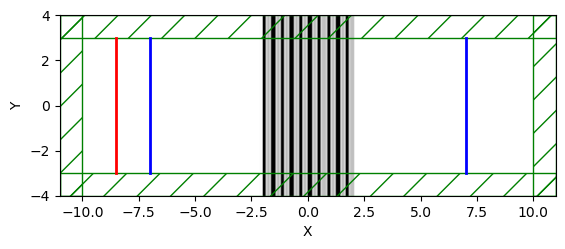
\includegraphics[width=0.8\linewidth]{Figures/bragg_design.png}
    \caption{Design of the simulation of a Bragg reflector. Structure composed of \(N=10\) layers and their widths are computed from Eq. \ref{eq:grating_period}. The simulation is done at resolution \(r=16\) and PML of thickness \(1\ \mu m\).}
    \label{fig:bragg_design}
\end{figure}

To measure the spectrum of this object, two detectors (blue lines in the figure) are used, one for the transmitted spectrum and one for the reflected one. The Bragg reflector is shined with a Gaussian source at wavelength \(\lambda = 1.55 \mu m\) and frequency width half of the central frequency. The reflector is designed to have this wavelength as the center of its spectrum and this is obtained by imposing the condition of constructive interference in the reflection. This corresponds to constructing the layers following Eq. \ref{eq:grating_period}  
\begin{equation}\label{eq:grating_period}
    n_1 L_1 = \frac{\lambda}{4} \qquad\qquad\qquad n_2 L_2 = \frac{\lambda}{4}
\end{equation}

The reflectance and transmittance spectrum are reported in Fig. \ref{fig:bragg_spectrum}, which shows a very low transmittance in a range of frequencies, paired with a high reflectance in the same range. Considering the transmitted spectrum this range of frequencies is a stop band and its borders are defined as the first maxima of the transmittance.

\begin{figure}[H]
    \centering
    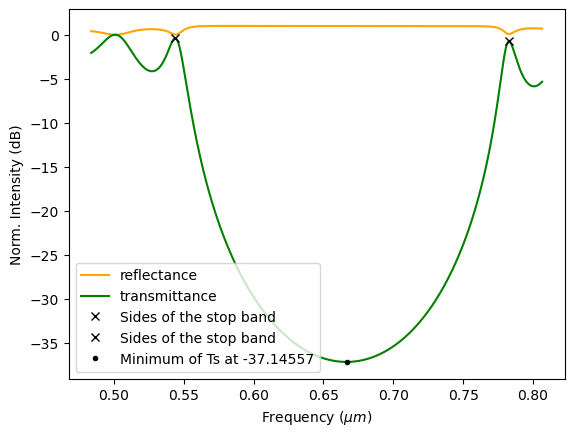
\includegraphics[width=0.6\linewidth]{Figures/bragg_spectrum.png}
    \caption{Transmission and reflection spectra of the Bragg reflector shined with a Gaussian source. The reflectivity and transmissivity are reported in dB to highlight how low is the transmittivity in the characteristic range of the Bragg reflector.}
    \label{fig:bragg_spectrum}
\end{figure}

The attenuation in the transmission depends on the refractive index contrast between the two materials and the number of layers as described by Eq. \ref{eq:attenuation}
\begin{equation} \label{eq:attenuation}
    T(\omega_0) \approx 4 \left(\frac{n_1}{n_2}\right)^{2N} 
\end{equation}
The result of the simulation is represented in Fig. \ref{fig:bragg_attenuation_vs_index} and it shows a good agreement with the fit, returning as a parameter the number of layers, compatible with the number set for the simulation, namely \(N=10\).

\begin{figure}[H]
    \centering
    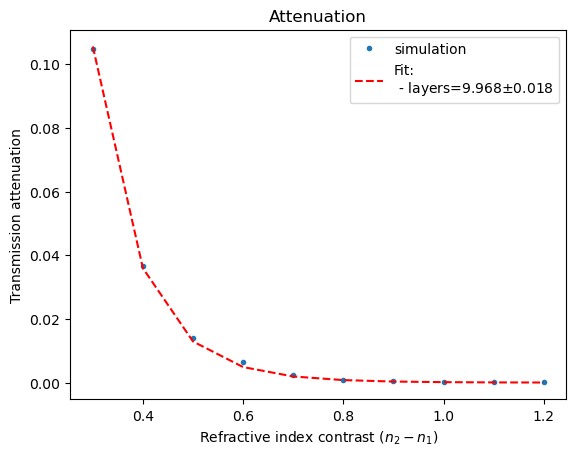
\includegraphics[width=0.6\linewidth]{Figures/bragg_attenuation_vs_index.png}
    \caption{Attenuation of the transmissivity as a function of the refractive indexes contrast. The simulation results are fitted with function in Eq. \ref{eq:attenuation} using as a free parameter the number of layers.}
    \label{fig:bragg_attenuation_vs_index}
\end{figure}

Mirrors made from Bragg reflectors reach a reflectance way higher than even the better metallic mirrors. They are the ideal mirrors for implementing a Fabry-Perot-like cavity, as the one represented in Fig. \ref{fig:bragg_cavity_design}.

\begin{figure}[H]
    \centering
    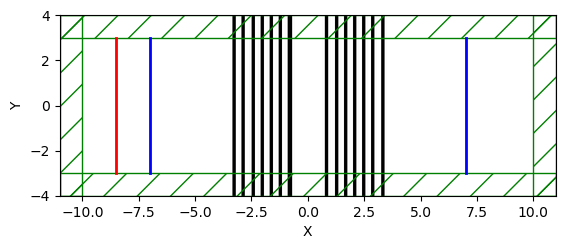
\includegraphics[width=0.8\linewidth]{Figures/bragg_cavity_design.png}
    \caption{Design of a Fabry-Perot cavity using Bragg reflectors instead of metallic mirrors. Each mirror is made of 7 layers and differently from the first simulation, the whole simulation space is made from a material of refractive index \(n_2 = 1.5\). The cavity is made from the material with a lower refractive index and it is \(1.5\ \mu m\) wide.}
    \label{fig:bragg_cavity_design}
\end{figure}

The presence of the cavity introduces a resonance in the system resulting in a different spectrum, with a peak in transmission in correspondence with this resonance, as shown in Fig. \ref{fig:bragg_vs_cavity_spectrum}. From this peak in the spectrum, it's possible to extract the Q-factor of the cavity, via a Lorentzian fit. The result of the fit is shown in Fig. \ref{fig:bragg_cavity_spectrum_fit} and returns a Q-factor\(=52\).

\begin{figure}[H]
    \centering
    \begin{subfigure}[b]{0.45\linewidth}
        \centering
        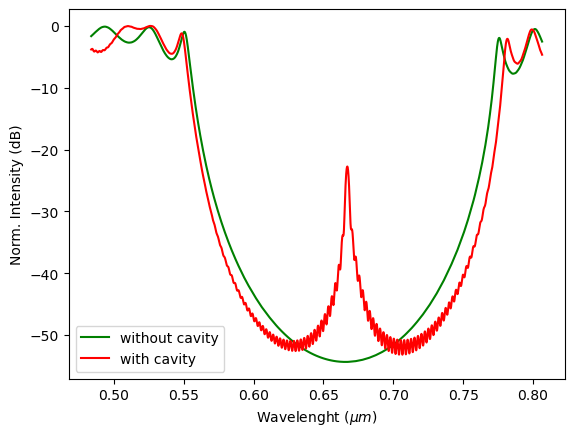
\includegraphics[width=\linewidth]{Figures/bragg_vs_cavity_spectrum.png}
        \caption{Comparison of the transmission spectrum of a Bragg reflector made of 14 layers and the transmission spectrum of a Fabry Perot cavity which uses Bragg reflectors, made of 7 layers, as mirrors.}
        \label{fig:bragg_vs_cavity_spectrum}
    \end{subfigure}
    \hfill
    \begin{subfigure}[b]{0.45\linewidth}
        \centering
        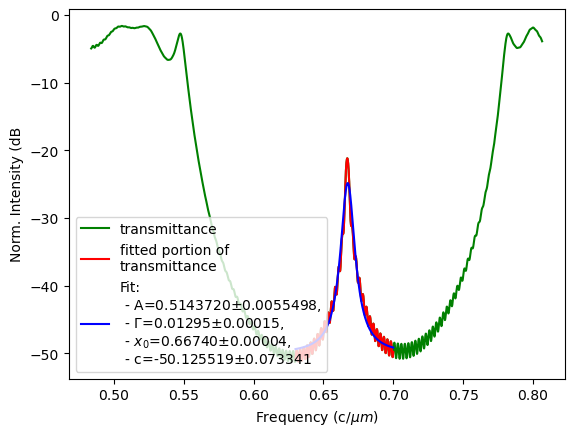
\includegraphics[width=\linewidth]{Figures/bragg_cavity_spectrum_fit.png}
        \caption{Lorentzian fit of the portion of the transmission spectrum of the cavity around the cavity's resonance to extract the Q-factor of the cavity.}
        \label{fig:bragg_cavity_spectrum_fit}
    \end{subfigure}
\end{figure}

The Q-factor depends on the quality of the mirrors, namely from the refractive index contrast between the layers, as shown in Fig. \ref{fig:bragg_cavity_qfactor_vs_index}, in fact, the quality factor of the cavity grows with the contrast, and so with the reflectivity of the mirrors.

\begin{figure}[H]
    \centering
    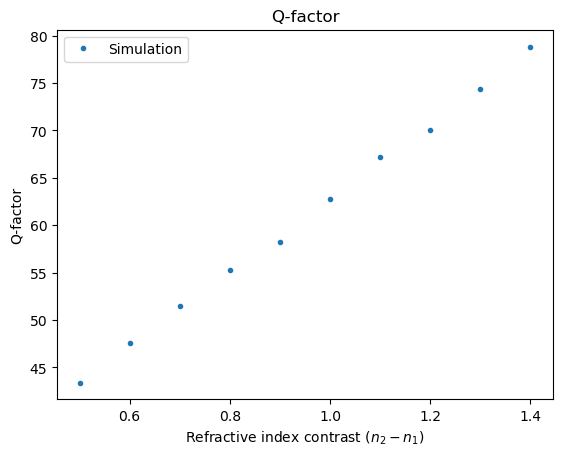
\includegraphics[width=0.6\linewidth]{Figures/bragg_cavity_qfactor_vs_index.png}
    \caption{Dependence of the Q-factor of the cavity from the reflectiveness of the mirrors, namely from the refractive index contrast between the layers forming the mirrors.}
    \label{fig:bragg_cavity_qfactor_vs_index}
\end{figure}